\documentclass[a4wide, 11pt]{article}
\usepackage{a4, fullpage}
\usepackage[hmargin=1.5cm,vmargin=1.5cm]{geometry}
\setlength{\parskip}{0.3cm}
\setlength{\parindent}{0cm}
\usepackage[T1]{fontenc}
\usepackage{longtable}
\usepackage{graphicx}
\usepackage{endnotes}
\setlength\LTleft\parindent
\setlength\LTright\fill
\linespread{1}


% This is the preamble section where you can include extra packages etc.

\begin{document}

\title{}

\author{}

\date{\today}         % inserts today's date

\begin{center}
  \ \\
  \ \\
  \ \\
  \ \\
  \ \\
  \ \\
  \ \\
  \ \\

\includegraphics[width=0.7\textwidth]{images/logo.png} \\ \ \\
Peter Hamilton, Sarah Tattersall, Niklas Hamb\"{u}chen, Lukasz Kmiecik
\ \\
\ \\
\ \\
\today
\end{center}
% \maketitle            % generates the title from the data above
\pagebreak

\tableofcontents

\pagebreak

\section{Introduction}
\subsection{Requirements and Targets}
We were asked to gain experience working as a group on a multi-part web programming project where we would learn all about client-side and server-side techniques and database usage.

\subsubsection{Specification Requirements}
There were several requirements our game was asked to meet, the main ones being:

\begin{itemize}
\item The game must run on at least one internet browser installed on lab machines
\item There must be a database
\item When a player logs out of a game his current state must be saved in a database so they can continue later
\item The game should allow players to send messages to each other
\item The game should be multiplayer
\end{itemize}

\subsubsection{Game Targets}
After reading the required specification, we came up with some additional targets that we wanted to achieve ourselves out of the game:
\begin{itemize}
\item The game should be real time and full of action
\item The game should involve more than two players and be cooperative
\item The game should be timed
\end{itemize}

\subsubsection{Personal Targets}
\begin{itemize}
\item
  Sarah (New to web development)
  \begin{itemize}
    \item Gain a basic understanding of client-server interactions
    \item Learn how to easily debug client-side errors
  \end{itemize}

\item
  Lukasz (New to web development)
  \begin{itemize}
    \item Further skills in web-based animations, graphics and user interfaces
  \end{itemize}

\item
  Niklas (Experienced in web development)
  \begin{itemize}
    \item Use already familiar technologies to make development as convenient as possible for the group; improve tooling skills
    \item Explore Github as a project management platform
  \end{itemize}

\item
  Peter (Experienced in web development)
  \begin{itemize}
    \item Explore new technologies such as NowJS, RaphaelJS, Mocha for Unit Testing
    \item Improve his CoffeeScript coding speed and quality
  \end{itemize}
\end{itemize}

\section{Project Management}
\subsection{Group Structure}
Instead of giving potentially constricting responsibilities to everyone in our group, we chose to use a more agile development strategy.
\\ \\
We maintained a working set of features and bugs that needed attention, hosted as part of our Github repository. These bugs and features were then assigned to the person who felt that the issue best matched their strengths and preferences.
\\ \\
Lukasz tended to take on graphics, UI and UX issues, Sarah prefered back end development such as the gameplay physics, Niklas usually tackled the real-time programming challenges and our development environment/setup, and Peter worked on both front and back end development where required ranging from turret control to code refactoring.

\subsection{Implementation Languages and Frameworks}
\subsubsection{Client and Server}
We use a number of technologies both client-side and server-side.

\begin{itemize}
  \item
    {\bf CoffeeScript}
    \footnote{http://coffeescript.org/}
    - Allows us to write Javascript in a really succinct and efficient way using a layer of beautiful syntactic sugar which compiles directly to JS. The result leads to faster, neater, more efficient javascript code.
  
  \item
    {\bf Mocha}
    \footnote{http://visionmedia.github.com/mocha/}
    - A behaviour-driven development (BDD) testing framework that lets us write elegant and understandable specifications of how different modules of our code shall behave. It runs on both node.js and the browser, unifying the way we write tests.
\end{itemize}


\subsubsection{Client Specific}
As we are targeting browsers, our game is written in HTML5, CSS3 and Javascript. Our real-time graphics are controlled with Rapha\"{e}l.js, and surrounding UI elements consist of old-school HTML styled with CSS.

\begin{itemize}
  \item
    {\bf Knockout.js}
    \footnote{http://knockoutjs.com/}
    Using "observable" variables, knockout can update all objects on the page automatically when javascript variables change. This allows us to skip manual DOM manipulation and write cleaner, simpler UI code.
  \item
    {\bf Stylus CSS}
    \footnote{http://learnboost.github.com/stylus/}
    - A styling language that compiles down to CSS. We decided to switch from vanilla css to Stylus to reduce code duplication. Styles are now more readable, concise and easier to edit.

  \item
    {\bf Rapha\"{e}l}
    \footnote{http://raphaeljs.com/}
    - A library for easily managing interactive SVGs, allowing manipulation of the contained objects with a simple-to-use JavaScript API. We use this for most of our graphics manipulations.

  \item
    {\bf gRapha\"{e}l}
    \footnote{http://g.raphaeljs.com/}
    - An extension of Rapha\"{e}l, allowing easy creation of graphs. When we decided on circular health indicators, we realised we could represent them as small pie charts using gRapha\"{e}l.

  \item
    {\bf Sonic js}
    \footnote{http://james.padolsey.com/javascript/sonic-looping-loaders/}
    - A small library that allows us to create customised loading animations. This allowed us to create spinners related to our theme.
  
  \item
    {\bf Vogue}
    \footnote{http://aboutcode.net/vogue/}
    - Refreshes our stylesheets live when they are changed, so that we don't have to restart the game to evaluate design changes.

\end{itemize}

\subsubsection{Server Specific}
Our server runs on \textbf{node.js} \footnote{http://nodejs.org/}, which means that we write Javascript in both the front-end and back-end of our game and that we can share common code (e.g. vector geometry) and frameworks, reducing code duplication.

\begin{itemize}
  \item
    {\bf NowJS}
    \footnote{http://nowjs.com/}
    For bidirectional communication between client and server. A transparent bridge that makes RPCs look like ordinary JavaScript functions. Based on Websockets, this is what makes our game real-time.
  
  \item
    {\bf MongoDB}
    \footnote{http://www.mongodb.org/}
    A NoSQL database we use for storing persistent information that exceeds the length of a game. The fact that it stores objects makes working with Javascript a breeze.

  \item
    {\bf Mongoose}
    \footnote{http://mongoosejs.com/}
    A convenient high-level mapper allowing node.js to communicate with our MongoDB database. The real-time game state is stored in-memory in our node application.
\end{itemize}

\subsection{Design Practices}

We were very strict from the beginning that our code should be easy to read and understand so that any of us could clearly grasp what was happening in any part of the system at any given time.

To ensure this we had a few best practices which we enforced as a group:

\begin{itemize}
\item
  Structured our code into classes, closely modelling the different elements of our game (e.g. Players, Turrets, Balls). This made sure everyone had a good overview and knew where to search for whatever piece of code.
\item
  Introduced a configuration file. This holds variables which are used throughout the code instead of being hard coded everywhere. It firstly makes the code more readable than having an unexplained number (e.g. \textit{max\_player\_health} instead of \textit{1.0}) and it also means that if we wish to change its assigned value we only have to change it in one place.
\item
  Commented all functions/methods/variables that were not entirely clear. This was particularly important so that we could all understand what other people had done and made it far easier to integrate our work with what someone else had done.
  \\
  We had a strict policy concerning this: As soon as there was a piece of code which a team member did not find entirely clear, the author of that code had to improve their comments on it until everybody understood.
\item
  We know from experience that growing projects can become very messy if they do not consistently follow a thought-out structuring concept, especially concerning the separation and interaction of game logic, state, networking and view components.
  This is particularly important in programming languages like Javascript, which basically allow doing everything everywhere.
  We chose a Model-View-Presenter pattern with an additional Networking Controller and strictly built on it from the beginning. In fact, we have two MVP-N instances:

  \begin{itemize}
  \item
    One on the client, with the Game class being the managing presenter, and view components such as \emph{Turret} and \emph{Arena}. Knockout's MVVM\footnote{Model-View-View-Model and Data Binding: http://en.wikipedia.org/wiki/Model\_View\_ViewModel} pattern further forced us to bind data into our HTML page in a rigorous way, exempting us from manual DOM updates.
  \item
    One on the server, where the \emph{Server} class interfaces with the \emph{ArenaModel} as the top level model component as well as with the client Presenters inside the connected browsers via RPCs\footnote{Remote Procedure Calls using NowJS}. The View part is a terminal output.
    
          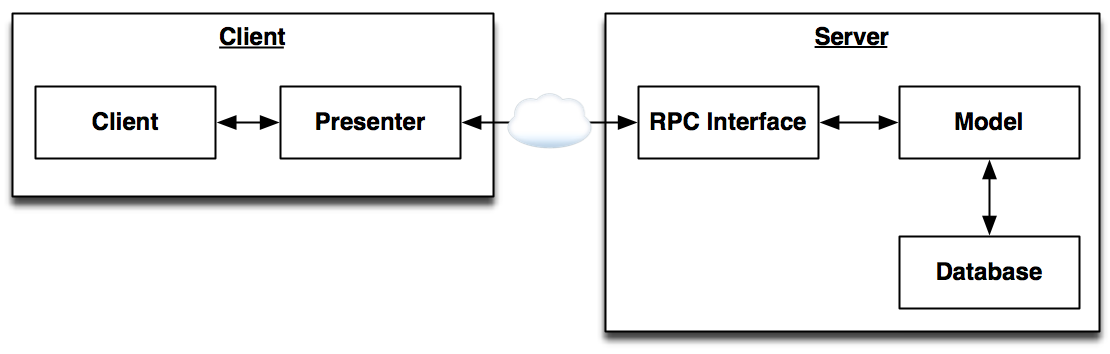
\includegraphics[width=0.9\textwidth]{images/simple_interaction.png} \\
  \end{itemize}

\item
  The client-server bridge is often not only an interface between different machines, but also between different developers. It is thus inherently error-prone. We considered it essential to make this interface absolutely clear and completely separated our networking code from the rest of the logic code. All RPCs are now bundled into a single place on each side (\emph{main.coffee} on the client and \emph{server.coffee} on the server), this means that client developers only have to know that single counterpart of the server, and all network traffic goes through that interface\footnote{This is similar to routing frameworks in stateless web applications}, which alleviates debugging.

\item
  Because our game runs in real-time, we had to make the important decision on how to synchronise how the game is going on between the server and the clients. There were basically two choices:
  \begin{itemize}
    \item
      Keeping a full game state in each client and letting it perform actions on that state quite independently. This requires synchronising the state with the server regularly to check if the client is still playing according to the game rules.
    \item
      Keeping the client close to state-less, and only sending over \emph{events} to the clients, which act accordingly.
  \end{itemize}
  
  We did not want to implement the first option, as "merging" diverged game states is usually very complicated and often leads to arbitrary resolution choices. Going for the second option, we potentially have to transmit more data (sending the actual values describing the events instead of simple acknowledgement messages). However, this form of evented programming gives us fine-grained control about which data we have to send (compared to syncing the full state), which allows us to keep our messages just as small as they need to be\footnote{And they do need to be small, as we send around 40 per second per player for a smooth, action-loaded experience. A typical message is around 50 bytes small, while we expect our full game state to occupy around 10 KB in JSON format.}.
\end{itemize}


\subsection{Code Management and Workflow}

Not only was using some sort of version control a requirement but we also felt strongly that it was very important for our development workflow.

Using version control allowed us all to work on the codebase together. We could easily regain previously deleted work without wasting time re-writing it. We could also work on new features independently without interfering with the master version of the codebase. Version control also provides useful logs and by forcing messages for commits it allows other users to quickly gain a brief overview of what another person done.

We decided to use Git over other version control systems such as Subversion because:
  \begin{itemize}
    \item
      It is fast as most operations are performed locally.
      
        \begin{center}
          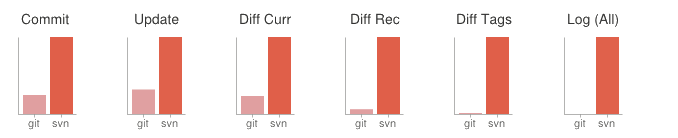
\includegraphics[width=0.9\textwidth]{images/git_compare.png} \\
          \emph{Performance comparison of Git and Subversion\footnote{http://git-scm.com/about/small-and-fast}, showing the operations we need most}
        \end{center}
        
    \item
      It allows for easy branching. This is very useful when we were creating new features, we could each work on a branch without interfering what our other team members were doing. We ensured we only merged into the master when the code was working.
    \item
      Git also allows us to work on our project whilst not on a network because the entire repository and history is stored on your computer. This allowed for us to code and more importantly commit, without necessarily being connected to the internet.
    \item
      We had all used git before and were already fairly proficient with it, so it did not cause unnecessary stress for us whilst coding our project.
  
  \end{itemize}

Once we knew we would use Git we decided to host our project codebase on Github\footnote{https://github.com/} because it has some very nice features:

  \begin{itemize}
    \item We could create a wiki
    \item We could create and track issues easily
    \item Our project is automatically backed up
  \end{itemize}

  We created a private project on Github (to be made open source after the project was more finalised) and then used our Wiki to document any thoughts and useful links we had for the game. We also created a "Plan of Action" page which involved several implementation phases. These were:
  

\begin{center}
  \begin{tabular}{ | l | l | }
    \hline
    
    Phase 1 - Setup & 
      Get everyone set up on git and using the same tools and languages \\
    \hline
    
    Phase 2 - Simple Proof of Concept & 
       Turret (movement only),
       Real time actions,
       Floating Plasma Balls \\
    \hline
    
    Phase 3 - Player Actions & 
       Grabbing balls,
       Shooting balls \\
    \hline
    
    Phase 4 - Shield/Health & 
       Diminishing shield,
       Player death \\
    \hline
    
    Phase 5 - Add another Player	 & 
       Shooting,
       Health Damage,
       Basic Scoring \\
    \hline
    
    Phase 6 - Multiplayer & 
      Game rooms,
      Lobby/Joining \\
    \hline
    
    Phase 7 - Additional Features & 
       Power ups,
       Turret Customisation \\
    \hline
    
    Phase 8 - Database Integration & 
       Scoring,
       Profiles,
       Login \\
    \hline
  \end{tabular}
\end{center}

With the exception of Phase 8 (the database), we pretty much stuck to this ordering, leaving the extra optional elements until last so that we could focus on the important things for the game.
We implemented a database earlier than we originally planned as it was useful for creating the lobby. We also did not want to leave it until last in case we encountered any problems.

To ensure everyone kept up to date on issues and bugs, we made sure to note everything, including relevant commit references and links to useful source material. The end result was a clear chain of comprehensive communication integrated tightly with our code and understandable by everyone. 

\begin{center}

  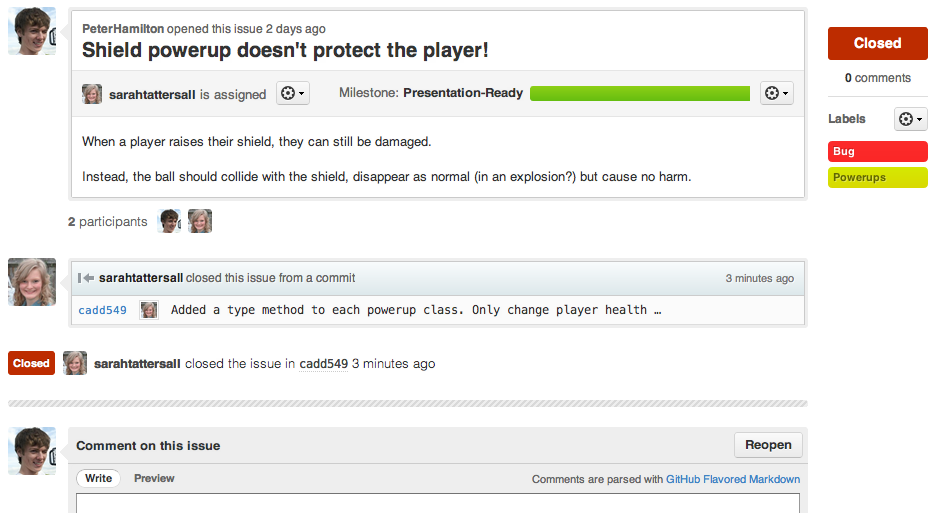
\includegraphics[width=0.9\textwidth]{images/git_issue.png} \\
  \emph{Workflow: A bug with discussion and the commit that fixed it.}
\end{center}
      
To ensure we didn't encounter any strange non-reproducible errors, we set up a series of scripts to help synchronise our development environments\footnote{For example: Fetch latest versions of libraries, initialise database, run development servers, run tests.}. This meant that everyone could call simple commands to download all the relevant libraries, install packages and set up the servers. A good example of this is we added an option to our makefile which allowed us to run "make test" before pushing our commits to ensure we had not broken any working code or features that other people had written, if we had we fixed them before pushing.

Our testing suite included tests to ensure that the ball positions were calculated correctly on the screen, tests to check the rotations of the balls were calculated correctly, and tests to ensure balls ended up where we expected them to be. An example of a test run can be seen below.

\begin{center}
    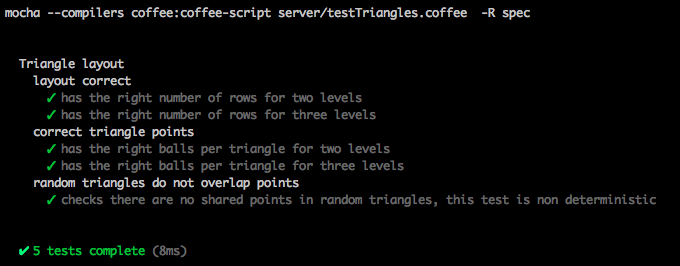
\includegraphics[width=0.9\textwidth]{images/test_run.png} \\
    \emph{Part of our BDD server testing}
\end{center}

Other examples of code we tested are collision detection, player functionality, database communication.

We also tried to carry out code reviews of each others work. When someone committed their work and pushed it up to the server another team member would normally read over it and point out potential problems. Praise was also given when we liked what someone had written. We found using code reviews helped with continuity of coding style. 

\section{Implementation}
\subsection{The Idea}
In order to decide on a game to implement we had a brain storming morning where we suggested all sorts of game such as logic games, shooting games, last man standing games. For the morning we allowed ideas to develop and flow without shooting down any suggestions as we were well aware that the first idea is not always the best. It was during lunch that we came up with our game idea: Gravitas, a real-time turret shooting game. We thought it would be exciting, engaging, and most importantly we felt it was feasible to implement in the time given.

\begin{center}

    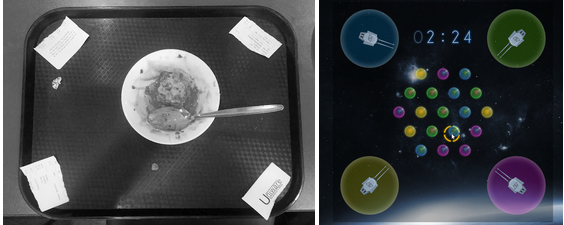
\includegraphics[width=0.9\textwidth]{images/game_lunch.png} \\
  \emph{Lunchtime brainstorming of the arena compared to the final design}
\end{center}

\subsection{How To Play}
Our game is based on a "Last Man Standing" mode of gameplay. Rounds are three minutes long and the time is indicated by the countdown timer on each player's game screen. In order to destroy an opponent each player must acquire plasma balls of their own colour from the moving plasma balls in the centre of the arena.

To acquire a plasma ball a player must have a clear line of sight (i.e. with no other balls in the way). If a player cannot reach a ball, or they click on a ball that is not their colour then we play an error sound so that it is clear they can't acquire it. However if the ball is acquirable then a player must hold down their mouse to obtain the ball and release it to fire at an enemy; both these actions implement pulling/releasing sounds for the individual player. 

Being hit by a plasma ball will cause a players health to decrease until they are left with nothing, at which point they die and must sit out for the rest of the round. As rounds are short players don't have to wait for too long until the end of the game.

To make things more interesting power ups have a 20\% chance of occurring when a ball is respawned in the centre. Power ups are kept a secret what type they are and as a player acquires a power up a message flashes up on their screen to tell them what they have received which none of the other players can see. They then are told they can press space at any time to activate it. By not immediately activating a power up it allows the player to save it for a time when they need it the most and allows for strategic hoarding of a power up.

The power ups available so far are a shield which makes the players field glow white whilst absorbing balls without damaging a players health and a full health power up. The shield only lasts for a few seconds, so as not to give an infinite advantage to a player, while the full health power up returns the player's health to what they had at the start.

We implemented a players health using a coloured field around each player. This field is useful to display how much health a player has (it shrinks on hit) and also because it is the colour of the balls they need to acquire. We hope this makes it intuitive for the players which balls they need to collect. Just before a player dies their shield glows red, which indicates they can only have one more hit before they die.

When a player dies all their balls will be removed from the centre of the arena so as not to clutter it with balls other players cannot acquire.

\begin{center}

    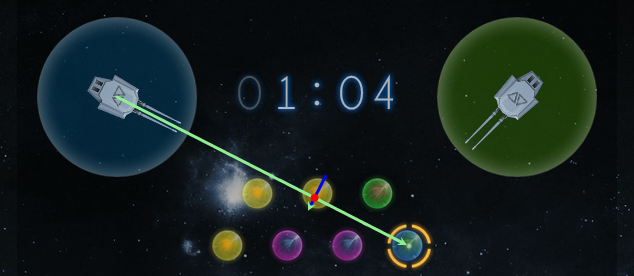
\includegraphics[width=0.9\textwidth]{images/shoot_collision.png} \\
  \emph{Two players with health fields and a ball striking one of them. Development visuals enabled.
You can also see the game timer counting down.}
\end{center}
\ \\
Finally when the game is over, either because time has run out or only one player has survived, the statistics are recorded to a database and all players return back to the lobby to start a new game.

Our game will also allow for player collaboration in two vs. two matches. The matches will be largely the same as the non-collaborative gameplay, with the addition that a player can fetch balls for their other teammate if they cannot reach it themselves. We hope that this makes the game more interesting for players and that they'd come back and play more often.

\section{Technical Challenges}
\subsection{Real Time Gameplay}
The real-time component of our game is based on event-driven development via NowJS RPCs.
\\ \\
Depicted below is the control flow that manages the movement of turrets: When a player moves the mouse, the corresponding turret shall move on the screens of all other players and the server-side model has to be updated.
\\ \\
Note the separation between the current user and “everyone else” as well as the MVP-N pattern mentioned earlier.

\begin{center}

    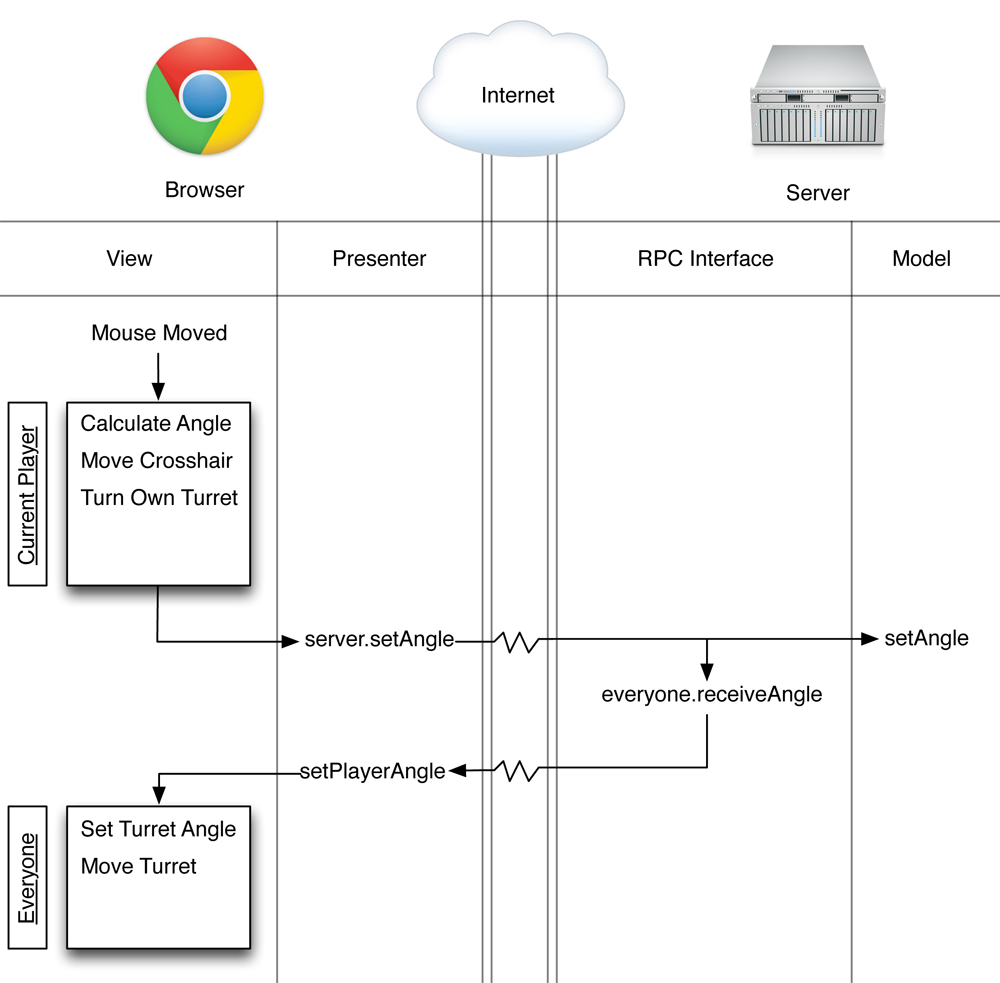
\includegraphics[width=0.7\textwidth]{images/mousemove_diag.png} \\
  \emph{Control Flow diagram for the movement of turrets}
\end{center}

\subsection{Ball Positioning}
To ensure constant movement and engagement in our game, we decided to make the balls in the centre of the game screen rotate around each other and swap positions. This required several stages of computation and had to maintain synchronisation across all connected client machines.

On the server side, we calculated the ball positions relative to the canvas and transformed them into a reduced coordinate grid. We then connected nearby points into triangles, generating an array containing every single possible combination of triangles for our ball coordinates (see step 2 below).

From this array, we selected a random number of disjoint triangles and stored them in a hash along with a rotation direction. This was done by picking a triangle from the list and filtering out any other triangles which shared a coordinate with it, repeating until the list is empty.

Each time the balls move the triangles and rotation directions are random, so the user has no idea which balls will move or which direction they will rotate.

Once the triangles had been selected, we were able to calculate the post-rotation ball positions, apply these new positions to the ball models and make a call to all clients to animate the ball views for the given models. This is done using a raphaelJS transform animation.

\begin{center}

    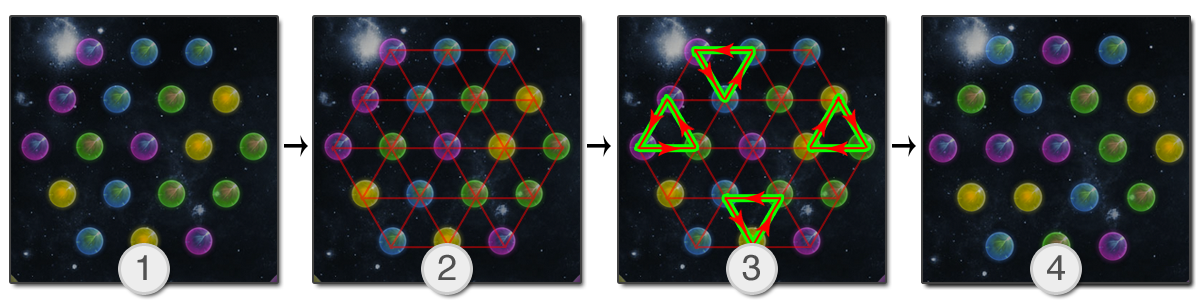
\includegraphics[width=0.9\textwidth]{images/triangles.png} \\
\end{center}

\subsection{Object Intersections}
During the course of our project we repeatedly found the need to work out if two objects intersected, lines, balls, turrets, shields and more.

To solve this we wrote our own minimal 2D vector library. We use this to determine whether one ball is in the way of another using segment intersections and also to check if a ball would hit a turret once it was fired along with where the impact point would be. To complement this library, we also implemented a debug mode that outputs elements in a browser which could show us what our physics engine was doing.

\begin{center}

    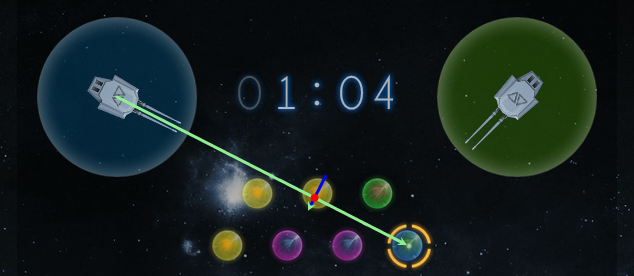
\includegraphics[width=0.9\textwidth]{images/shoot_block.png} \\
    \emph{Player attempting to pull a ball that they can't reach}
\end{center}

Once a ball has been fired, the server makes a call to the clients, passing them the impact point (or another point off screen). The client then uses RaphaelJS' animate method with callback functions to handle the graphics once the ball collides with the turret e.g dissolve, explode, decrease health etc. We used animation callbacks because otherwise the function would be called immediately after the initial animation call and not when the animation was finished.

\section {Game Interfaces}
\subsection{Profile and Lobby}
When the players are not engaged in a mind-blowing turret battle, they can enjoy the less violent parts of our game. A player is able to modify their profile, chat with other players, find their friends, view their gameplay statistics and more. There are also several leader boards which players can compete on based upon different criteria and challenges.

\subsubsection{Profile Screen}
Players each have their own profile page on the website that other players can view. It holds basic information, gameplay statistics, a global score and a profile picture.

The gameplay statistics are displayed in visually appealing, interactive graphs and the global score in the top right is coloured to their particular level and changes as they progress. Using little dynamic elements like these really help with increasing user engagement.

\begin{center}

    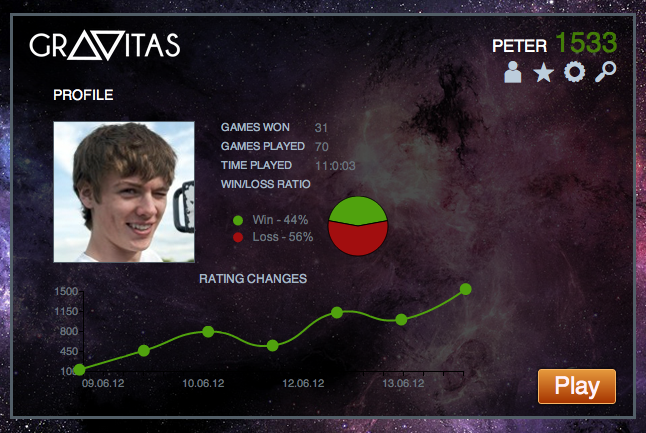
\includegraphics[width=0.7\textwidth]{images/profile.png} \\
  \emph{A player's profile showing their performance is developing positively during the last week.}
\end{center}

\subsubsection{Achievements Screen}
After players have achieved certain noticeable goals in the game, they awarded special trophies which are displayed as Achievements in their profiles and visible to others.
We have added some basic achievements at the time of writing, \emph{such as winning one game}, \emph{winning 100 games} and\emph{ playing for 10 hours}, and there is room for many more, especially ones that accredit the use of sophisticated tactics (e.g. collaborative ball passing or just-in-time shield usage).

\begin{center}

    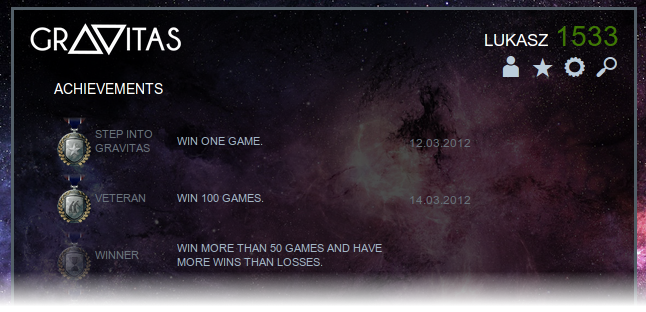
\includegraphics[width=0.7\textwidth]{images/acheivement.png} \\
  \emph{An achievement screen showing that the player has already won over 100 games}
\end{center}

\subsubsection{Settings Screen}
Users can view their player information such as in-game name and email address, change their password, and, more importantly, upload custom avatars to give the game a more personal touch.

\begin{center}

    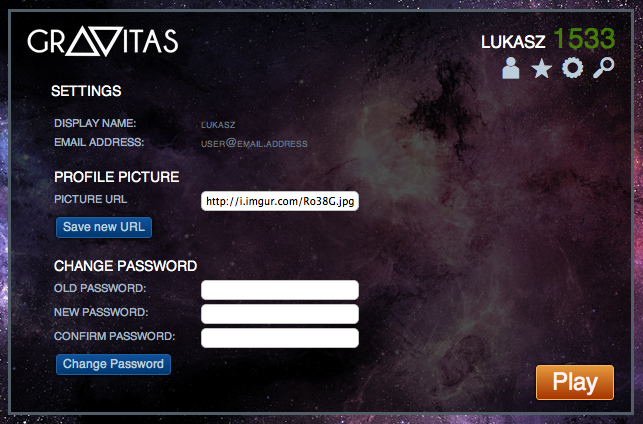
\includegraphics[width=0.7\textwidth]{images/settings.png} \\
  \emph{A player's settings screen showing the various options they could change}
\end{center}


\subsubsection{Search Screen}
Every user can display the profiles of others to compare score, statistics and other information with their own.


\begin{center}

  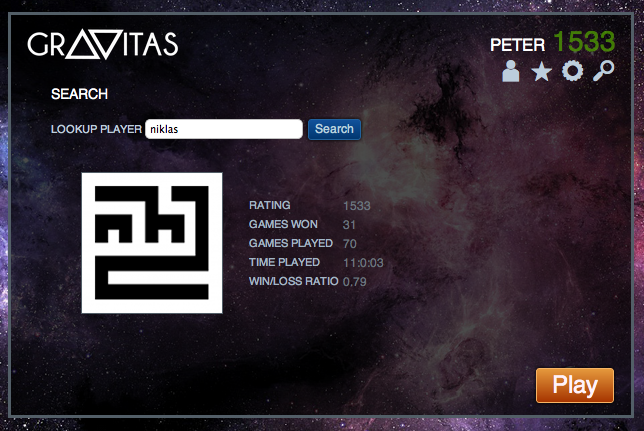
\includegraphics[width=0.7\textwidth]{images/search.png} \\
  \emph{The search screen where players can find their friends}
\end{center}

\subsubsection{Lobby}
Once a player has inspected their profile and configured their settings to their favour, they can advance to the Lobby, where they gather up to groups of four and start a game as soon as everyone is ready.

The lobby shows the other players waiting\footnote{The waiting is symbolised in the UI using a custom made throbber featuring two spinning triangles (the logo of Gravitas) which we are disproportionately proud of.} to enter the game and also features a chat to them to keep them engaged. Besides each player, their ranking is shown to avoid frustrating games between players of too unbalanced skill levels.
The lobby shows the other players waiting\footnote{The waiting is symbolised in the UI using a custom made throbber featuring two spinning triangles (the logo of Gravitas) which we are disproportionately proud of.} to enter the game and also features a chat to them to keep them engaged. Besides each player, their ranking is shown to avoid frustrating games between players of too unbalanced skill levels.


\begin{center}

    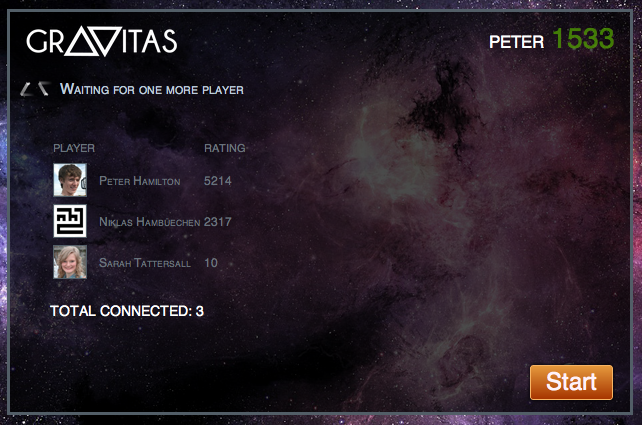
\includegraphics[width=0.7\textwidth]{images/lobby.png} \\
    \emph{The lobby screen where players wait for players before starting }
\end{center}

\section{Acknowledgements}
\subsection{Code}
Code that was not written by us has had its links referenced throughout.

\subsection{Sounds}
\begin{itemize}
    \item Health power up was the Skype sign in noise
    \item Disallowing of pulling other player balls is Apple's Funk sound for OS X
    \item Our shield power up comes from the shield suit power up of Half Life 2
    \item The pulling and shooting noises of each players "gravity gun" comes from the gravity gun sound from Half Life 2 also.
\end{itemize}

\subsection{Images}
\begin{itemize}
    \item Our lobby background image was taken from a Galaxy Ace wallpaper\footnote{http://www.pickywallpapers.com/1680x1050/space/galaxy-ace-wallpaper/}
    \item Our gameplay background was a modified space wallpaper\footnote{
http://www.hd1080wallpaper.com/wallpaper/sunrise-space-planets-hd-wallpaper.html}. We change the colour and removed a planet.
    \item We created our Gravitas logo, turrets and plasma balls ourselves.
\end{itemize}

Furthermore, if we wish to release this game in the future we will make sure that all the graphics/sounds are in the public domain or created by ourselves so as to not infringe on any copyright issues. 

\section{Conclusion}
\subsection{Summary and Learning Outcomes}
Over the course of the last few weeks we have created a fun game from scratch.
We think we have made good use of this project to improve our communication and project management skills and have expanded our programming skills with Javascript, CoffeeScript, CSS and Mongo.
We got a good grasp at what it is like to do web development and design in a small team, and we honestly enjoyed it. Each of us feels that they reached a deeply satisfying level of proficiency in the technologies we used most, and at the same time feel capable of setting up a full web application stack on our own if required.

\subsection{Further Improvements}
If we had had more time there are several improvements we would like to have made on our game:
\begin{itemize}
    \item\textbf{Even better plasma ball rotations -} Although the triangle method is good, some balls do not rotate on a single iteration of the algorithm, this is because you cannot possibly rotate all balls without having some overlapping. A better improvement would be to allow other shapes such as squares, and triangles that are not necessarily one hop away from each other. This algorithm would be more complex and we decided that the game is in a playable state as it is currently.
    \item\textbf{Power ups -} We would very much have liked to create more power ups, such as the ability to pull any ball, double damage etc. This would add more variety to the game.
    \item\textbf{Mobile Version -} Our game already works quite well on tablet browsers however there is still room for improvement especially for smaller screens and processing touch input.
    
\end{itemize}


\end{document}



































